\chapter{Resultados}
\label{cap:resultados}

% Rascunho em tópicos (2026-10-22). Números: \result{} de ../generated (agrupado nos
% três vídeos, média ± meia-largura do IC de 95% bootstrap por track, quando houver).
% As tabelas vêm prontas de ../generated (cabeçalhos em inglês).

\section{E0: instrumentos}
\begin{itemize}
\item TAR a FAR 1\%, FaceNet: demo1 \result{e0/demo1/facenet.tar}; demo2 \result{e0/demo2/facenet.tar}; demo3 \result{e0/demo3/facenet.tar}.
\item TAR a FAR 1\%, ArcFace: \result{e0/demo1/arcface.tar}; \result{e0/demo2/arcface.tar}; \result{e0/demo3/arcface.tar}.
\item demo1 é um teste fraco (rostos menores e mais virados).
\item Mix nativo do FaceFusion: a direção que ele subtrai é quase ortogonal à pretendida (cosseno médio \result{e0/mechanism/emap-direction-cos-mean}), porque a matriz \texttt{emap} está longe de ortogonal (\result{e0/mechanism/emap-orthogonality}).
\item Pisos de ruído (quadros reais consecutivos): expressão \result{e0/noise/expression}; pose \result{e0/noise/pose_err}\textdegree; $\kappa$ \result{e0/noise/emotion_kappa}; idade \result{e0/noise/age_err} anos; gênero \result{e0/noise/gender_agree}.
\item O probe de gênero troca de classe entre quadros consecutivos da mesma pessoa em $1 - \result{e0/noise/gender_agree}$ dos casos.
\end{itemize}

\begin{table}[ht]\centering
\caption{E0: limiar in-domain e TAR a FAR 1\% por vídeo e reconhecedor.}
% generated by experiments/e0_instruments/run.py — do not edit
\begin{tabular}{llrrrrr}
\toprule
Video & Recognizer & Threshold & TAR & Genuine & Impostor & Pairs \\
\midrule
demo1 & FaceNet & 0.776 & 0.353 & 0.649 & 0.282 & 436/2300 \\
demo1 & ArcFace & 0.471 & 0.587 & 0.531 & 0.057 & 436/2300 \\
demo2 & FaceNet & 0.777 & 0.692 & 0.808 & 0.331 & 996/10500 \\
demo2 & ArcFace & 0.527 & 0.795 & 0.672 & 0.158 & 996/10500 \\
demo3 & FaceNet & 0.713 & 0.731 & 0.785 & 0.285 & 1327/17450 \\
demo3 & ArcFace & 0.531 & 0.741 & 0.661 & 0.163 & 1327/17450 \\
\bottomrule
\end{tabular}

\end{table}

\section{E1: detecção}
\begin{itemize}
\item SCRFD-10GF, AP hard \result{e1/widerface/scrfd-10gf/ap-hard} (publicado para a variante com keypoints: 0,828). Valida o porte do protocolo.
\item SCRFD-34GF: AP hard \result{e1/widerface/scrfd-34gf/ap-hard}; latência \result{e1/widerface/scrfd-34gf/latency-ms}\,ms contra \result{e1/widerface/scrfd-10gf/latency-ms}\,ms.
\item YOLO-FaceV2-s: AP hard \result{e1/widerface/yolo-facev2-s/ap-hard}; recall a 0,1 FPPI \result{e1/widerface/yolo-facev2-s/recall-at-fppi-0.1} contra \result{e1/widerface/scrfd-10gf/recall-at-fppi-0.1}; latência \result{e1/widerface/yolo-facev2-s/latency-ms}\,ms.
\item Nos vídeos, YOLO-FaceV2-s acha mais rostos por quadro (demo2: \result{e1/demo2/yolo-facev2-s/faces-per-frame} contra \result{e1/demo2/scrfd-10gf/faces-per-frame}); não se sabe se as caixas extras são rostos.
\item Decisão: SCRFD-10GF em E2--E5 (licença do YOLO-FaceV2, derivado do YOLOv5, não verificada; todos os braços compartilham as detecções).
\end{itemize}

\begin{table}[ht]\centering
\caption{E1: WIDER FACE val, AP oficial e custo.}
% generated by experiments/e1_detection/run.py — do not edit
\begin{tabular}{lrrrrr}
\toprule
Detector & AP easy & AP medium & AP hard & Latency (ms) & Params (M) \\
\midrule
SCRFD-10GF & 0.949 & 0.935 & 0.813 & \textbf{21.540} & 4.230 \\
SCRFD-34GF & 0.959 & 0.947 & 0.840 & 40.670 & 9.780 \\
YOLO-FaceV2-s & \textbf{0.987} & \textbf{0.973} & \textbf{0.894} & 177.330 & 7.050 \\
\bottomrule
\end{tabular}

\end{table}

\section{E2: geradores na forma publicada}
\begin{itemize}
\item FaceNet rank-1, BLANKET (código liberado):
  \begin{itemize}
  \item rostos gerados \result{e2/pooled/blanket/generated/facenet.rank1};
  \item todos os rostos, passthrough como vazamento \result{e2/pooled/blanket/facenet.rank1} (gera só \result{e2/pooled/blanket/anonymized} dos rostos);
  \item vídeo final \result{e2/pooled/blanket/facenet_final.rank1}.
  \end{itemize}
\item GANonymization: gera \result{e2/pooled/ganonymization/anonymized}; todos \result{e2/pooled/ganonymization/facenet.rank1}; final \result{e2/pooled/ganonymization/facenet_final.rank1}.
\item Vídeo final: blur \result{e2/pooled/blur/facenet_final.rank1}; CIAGAN \result{e2/pooled/ciagan/facenet_final.rank1}; mosaico \result{e2/pooled/mosaic/facenet_final.rank1}.
\item A ordem dos métodos muda com a visão: como publicado, BLANKET é o menos privado; no vídeo final, não.
\item Utilidade nos rostos gerados, BLANKET: expressão \result{e2/pooled/blanket/generated/expression}; pose \result{e2/pooled/blanket/generated/pose_err}\textdegree; $\kappa$ \result{e2/pooled/blanket/generated/emotion_kappa}; gênero \result{e2/pooled/blanket/generated/gender_agree}; re-detecção \result{e2/pooled/blanket/generated/redetected}.
\item Censura e GANs: $\kappa$ perto de zero (CIAGAN \result{e2/pooled/ciagan/generated/emotion_kappa}; blur \result{e2/pooled/blur/generated/emotion_kappa}); pose 13--17\textdegree.
\item GANonymization: erro de idade \result{e2/pooled/ganonymization/generated/age_err} anos (desvio para mais velho).
\item Nenhum método chega perto do piso de emoção ($\kappa$ \result{e2/pooled/_noise_floor/generated/emotion_kappa}); identidades sintéticas do BLANKET tendem a sorrir.
\item Rostos $\ge 96$\,px: BLANKET os reidentifica quase sempre (Tab.~\ref{tab:r-e2-size}).
\item Custo (quadros/s): blur \result{e2/pooled/blur/fps}; mosaico \result{e2/pooled/mosaic/fps}; CIAGAN \result{e2/pooled/ciagan/fps}; GANonymization \result{e2/pooled/ganonymization/fps}; BLANKET \result{e2/pooled/blanket/fps} (processo principal em CPU; ver E5).
\end{itemize}

\begin{table}[ht]\centering
\caption{E2: cobertura e FaceNet rank-1 nas três visões, redução relativa e verificação no vídeo final.}
% generated by experiments/e2_generation/run.py — do not edit
\begin{tabular}{@{}l@{\hspace{5pt}}r@{\hspace{5pt}}r@{\hspace{5pt}}r@{\hspace{5pt}}r@{\hspace{5pt}}r@{\hspace{5pt}}r@{}}
\toprule
Arm & Coverage & R1 gen. & R1 all & R1 final & PG final & Verified \\
\midrule
blur & 1.00\,{\scriptsize$\pm$.00} & 0.07\,{\scriptsize$\pm$.05} & 0.07\,{\scriptsize$\pm$.05} & \textbf{0.07\,{\scriptsize$\pm$.05}} & 0.92\,{\scriptsize$\pm$.06} & 0.01\,{\scriptsize$\pm$.01} \\
mosaic & 1.00\,{\scriptsize$\pm$.00} & 0.12\,{\scriptsize$\pm$.06} & 0.12\,{\scriptsize$\pm$.06} & 0.12\,{\scriptsize$\pm$.06} & 0.87\,{\scriptsize$\pm$.07} & 0.02\,{\scriptsize$\pm$.01} \\
ciagan & 1.00\,{\scriptsize$\pm$.00} & 0.08\,{\scriptsize$\pm$.04} & 0.08\,{\scriptsize$\pm$.04} & 0.08\,{\scriptsize$\pm$.04} & 0.91\,{\scriptsize$\pm$.05} & \textbf{0.00\,{\scriptsize$\pm$.00}} \\
ganonymization & 0.47\,{\scriptsize$\pm$.10} & 0.10\,{\scriptsize$\pm$.06} & 0.51\,{\scriptsize$\pm$.10} & 0.09\,{\scriptsize$\pm$.04} & 0.90\,{\scriptsize$\pm$.04} & 0.03\,{\scriptsize$\pm$.02} \\
blanket & 0.28\,{\scriptsize$\pm$.12} & 0.48\,{\scriptsize$\pm$.16} & 0.77\,{\scriptsize$\pm$.07} & 0.15\,{\scriptsize$\pm$.08} & 0.84\,{\scriptsize$\pm$.09} & 0.02\,{\scriptsize$\pm$.02} \\
\bottomrule
\end{tabular}

\end{table}

\begin{table}[ht]\centering
\caption{E2: utilidade nos rostos gerados e piso de ruído.}
% generated by experiments/e2_generation/run.py — do not edit
\begin{tabular}{@{}l@{\hspace{5pt}}r@{\hspace{5pt}}r@{\hspace{5pt}}r@{\hspace{5pt}}r@{\hspace{5pt}}r@{\hspace{5pt}}r@{}}
\toprule
Arm & Expr. & Pose (\textdegree{}) & Emotion $\kappa$ & Age (y) & Gender & Re-det. \\
\midrule
blur & 0.28\,{\scriptsize$\pm$.04} & 17.18\,{\scriptsize$\pm$1.98} & -0.01\,{\scriptsize$\pm$.02} & 7.62\,{\scriptsize$\pm$1.25} & 0.45\,{\scriptsize$\pm$.08} & 0.00\,{\scriptsize$\pm$.00} \\
mosaic & 0.23\,{\scriptsize$\pm$.05} & 16.98\,{\scriptsize$\pm$1.94} & 0.03\,{\scriptsize$\pm$.10} & 12.56\,{\scriptsize$\pm$1.99} & 0.64\,{\scriptsize$\pm$.07} & 0.00\,{\scriptsize$\pm$.00} \\
ciagan & 0.21\,{\scriptsize$\pm$.05} & 14.19\,{\scriptsize$\pm$1.75} & 0.06\,{\scriptsize$\pm$.04} & 5.92\,{\scriptsize$\pm$1.09} & 0.41\,{\scriptsize$\pm$.09} & 0.95\,{\scriptsize$\pm$.04} \\
ganonymization & 0.14\,{\scriptsize$\pm$.02} & 13.16\,{\scriptsize$\pm$1.63} & 0.08\,{\scriptsize$\pm$.07} & 31.89\,{\scriptsize$\pm$4.34} & 0.67\,{\scriptsize$\pm$.09} & 0.54\,{\scriptsize$\pm$.10} \\
blanket & 0.11\,{\scriptsize$\pm$.05} & 7.30\,{\scriptsize$\pm$2.29} & 0.12\,{\scriptsize$\pm$.10} & 5.65\,{\scriptsize$\pm$1.62} & 0.83\,{\scriptsize$\pm$.09} & 0.99\,{\scriptsize$\pm$.01} \\
Real, next frame & \textbf{0.03\,{\scriptsize$\pm$.01}} & \textbf{1.99\,{\scriptsize$\pm$.37}} & \textbf{0.86\,{\scriptsize$\pm$.05}} & \textbf{1.18\,{\scriptsize$\pm$.19}} & \textbf{0.94\,{\scriptsize$\pm$.02}} & -- \\
\bottomrule
\end{tabular}

\end{table}

\begin{table}[ht]\centering
\caption{E2: FaceNet rank-1 nos rostos gerados por tamanho do rosto.}
\label{tab:r-e2-size}
% generated by experiments/e2_generation/run.py — do not edit
\begin{tabular}{@{}l@{\hspace{5pt}}r@{\hspace{5pt}}r@{\hspace{5pt}}r@{}}
\toprule
Face size (px) & 0–48 & 48–96 & $\geq$96 \\
\midrule
blur & 0.06\,{\scriptsize$\pm$.05} & 0.07\,{\scriptsize$\pm$.08} & 0.11\,{\scriptsize$\pm$.16} \\
mosaic & 0.08\,{\scriptsize$\pm$.06} & 0.17\,{\scriptsize$\pm$.11} & 0.14\,{\scriptsize$\pm$.19} \\
ciagan & 0.07\,{\scriptsize$\pm$.04} & 0.05\,{\scriptsize$\pm$.04} & 0.22\,{\scriptsize$\pm$.26} \\
ganonymization & 0.13\,{\scriptsize$\pm$.08} & 0.06\,{\scriptsize$\pm$.05} & 0.11\,{\scriptsize$\pm$.16} \\
blanket & 0.37\,{\scriptsize$\pm$.19} & 0.34\,{\scriptsize$\pm$.14} & 0.97\,{\scriptsize$\pm$.05} \\
\bottomrule
\end{tabular}

\end{table}

\section{E3: contribuição}

\subsection{C2 (E3a)}
\begin{itemize}
\item Cosseno com a segunda metade do track: média \result{e3a/pooled/mean.heldout-cos}; média ponderada \result{e3a/pooled/quality_mean.heldout-cos}; melhor quadro \result{e3a/pooled/best.heldout-cos}; primeiro quadro \result{e3a/pooled/first.heldout-cos}; EMA \result{e3a/pooled/ema_adaptive.heldout-cos}.
\item Referência entre pessoas diferentes (tracks no mesmo quadro): \result{e3a/pooled/cross-track-cos-mean}.
\item O track estima melhor que um quadro; os pesos de qualidade definidos à mão não ajudam.
\item Como alvo do P2 (E3d), nenhum modo supera o primeiro quadro (média ponderada: \result{e3d/pooled/quality_mean/delta-facenet.rank1}, intervalo inclui zero).
\end{itemize}

\subsection{Cobertura (E3b)}
\begin{itemize}
\item Gerados: original \result{e3b/pooled/original/anonymized}; \emph{seed candidates} \result{e3b/pooled/candidates/anonymized}; detecção do Estágio~1 \result{e3b/pooled/phase1/anonymized}.
\item Vídeo final: \result{e3b/pooled/original/facenet_final.rank1} $\to$ \result{e3b/pooled/phase1/facenet_final.rank1}. Rosto oculto nunca é reidentificado; rosto trocado às vezes é.
\item $\kappa$: \result{e3b/pooled/original/emotion_kappa} $\to$ \result{e3b/pooled/phase1/emotion_kappa}. Cobertura total é o que mantém o comportamento.
\end{itemize}

\subsection{P2 (E3c)}
\begin{itemize}
\item FaceNet rank-1 (rostos gerados): mix nativo \result{e3c/pooled/native/facenet.rank1}; sem mix \result{e3c/pooled/none/facenet.rank1}; $\beta$ 1,2 \result{e3c/pooled/b-1.2/facenet.rank1}; $\beta$ 1,6 \result{e3c/pooled/b-1.6/facenet.rank1}.
\item $\Delta$ contra o nativo: $\beta$ 1,2 \result{e3c/pooled/b-1.2/delta-facenet.rank1}~$\pm$~\result{e3c/pooled/b-1.2/delta-facenet.rank1.ci}; $\beta$ 1,6 \result{e3c/pooled/b-1.6/delta-facenet.rank1}~$\pm$~\result{e3c/pooled/b-1.6/delta-facenet.rank1.ci}; todo $\beta \ge 0{,}35$ exclui zero.
\item Mix nativo indistinguível de nenhum mix (\result{e3c/pooled/none/delta-facenet.rank1}).
\item ArcFace rank-1: \result{e3c/pooled/native/arcface.rank1} $\to$ \result{e3c/pooled/b-1.2/arcface.rank1} (satura em $\beta$ 1,2; \result{e3c/pooled/b-1.6/arcface.rank1} em 1,6). O FaceNet vê cerca de um terço da queda.
\item Expressão (\result{e3c/pooled/native/expression} $\to$ \result{e3c/pooled/b-1.6/expression}) e pose (\result{e3c/pooled/native/pose_err} $\to$ \result{e3c/pooled/b-1.6/pose_err}\textdegree) estáveis.
\item $\kappa$: \result{e3c/pooled/native/emotion_kappa} $\to$ \result{e3c/pooled/b-1.6/emotion_kappa} (intervalos se sobrepõem).
\end{itemize}

\begin{figure}[ht]\centering
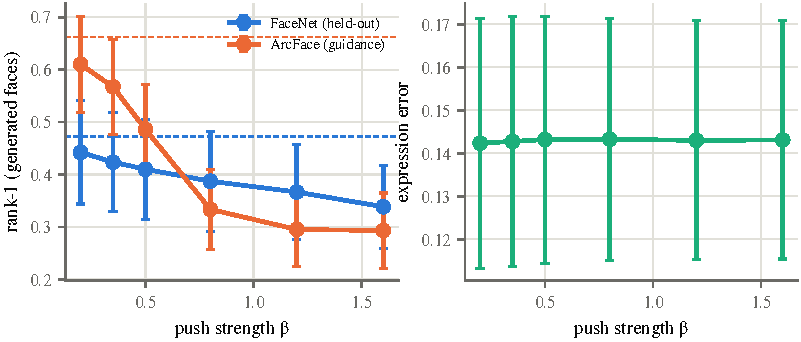
\includegraphics[width=\linewidth]{generated/e3_contribution/fig-e3-p2-curve}
\caption{E3c: rank-1 (FaceNet, ArcFace) e erro de expressão contra $\beta$; tracejado: mix nativo.}
\end{figure}

\subsection{Políticas (E3e)}
\begin{itemize}
\item Vídeo final, sobre P2 $\beta$ 1,2: P2 \result{e3e/pooled/p2/facenet_final.rank1}; \emph{hide-low} \result{e3e/pooled/hide-low/facenet_final.rank1}; \emph{gate} \result{e3e/pooled/gate/facenet_final.rank1}; ambos excluem zero.
\item Gerados: \emph{gate} \result{e3e/pooled/gate/anonymized}; \emph{hide-low} \result{e3e/pooled/hide-low/anonymized}.
\item Verificação: \emph{gate} \result{e3e/pooled/gate/facenet_final.verified} (a menor); \emph{hide-low} \result{e3e/pooled/hide-low/facenet_final.verified}.
\item Utilidade dos rostos mostrados: inalterada.
\end{itemize}

\subsection{P1 (E3g), negativo}
\begin{itemize}
\item FaceNet rank-1: \result{e3g/pooled/P1-c-0.1-+-P2/facenet.rank1} contra \result{e3g/pooled/P2/facenet.rank1} (P2 só); $\Delta$ \result{e3g/pooled/P1-c-0.1-+-P2/delta-facenet.rank1}~$\pm$~\result{e3g/pooled/P1-c-0.1-+-P2/delta-facenet.rank1.ci}, inclui zero.
\item Dentro do passo base, funciona: cosseno $\hat{x}_0$--real \result{e3g/pooled/guided-cos.p1-c0.1.first} $\to$ \result{e3g/pooled/guided-cos.p1-c0.1.last} (\result{e3g/pooled/guided-cos.p1-c0.1.identities} identidades).
\item Na imagem de identidade final: \result{e3g/pooled/identity-cos.p1-c0.1} com P1 contra \result{e3g/pooled/identity-cos.plain} sem (mediana pareada \result{e3g/pooled/identity-cos.p1-c0.1.paired-median}).
\item Onde se perde: último passo base, decodificação e refiner (img2img só com o prompt). O resto chega à troca só pelo embedding, que P2 já empurra.
\end{itemize}

\subsection{P3 (E3f), negativo}
\begin{itemize}
\item $\Delta$ FaceNet rank-1: \result{e3f/pooled/P3-tau-0.0/delta-facenet.rank1} ($\tau = 0$), \result{e3f/pooled/P3-tau--0.2/delta-facenet.rank1} ($\tau = -0{,}2$).
\item CIAGAN puro já perto do acaso: \result{e3f/pooled/ciagan/facenet.rank1}.
\item \emph{Hinge} ativa em \result{e3f/pooled/P3-tau-0.0/push.active} ($\tau = 0$) e \result{e3f/pooled/P3-tau--0.2/push.active} ($\tau = -0{,}2$) dos rostos.
\item Cosseno: \result{e3f/pooled/P3-tau-0.0/push.cos-start} $\to$ \result{e3f/pooled/P3-tau-0.0/push.cos-end}; massa no código da seed \result{e3f/pooled/P3-tau-0.0/push.p-seed}.
\item O otimizador não move o código: penalidade do pseudônimo, gradiente plano do softmax, pouca variação de identidade dentro do casco.
\end{itemize}

\section{E5: custo}
\begin{itemize}
\item ms por rosto: \emph{ref-cpu} \result{e5/pooled/ref-cpu/ms-per-face}; \emph{ref} \result{e5/pooled/ref/ms-per-face}.
\item Segmentação de cabeça: \result{e5/pooled/ref-cpu/stage-seg-ms}\,ms na CPU contra \result{e5/pooled/ref/stage-seg-ms}\,ms na GPU. Sem diferença pareada em privacidade ou utilidade.
\item Estágios por rosto gerado (\emph{ref}): GFPGAN \result{e5/pooled/ref/stage-gfpgan-ms}\,ms; landmarks \result{e5/pooled/ref/stage-landm-ms}\,ms; troca \result{e5/pooled/ref/stage-swap-ms}\,ms. PNG e RPC $\sim$10\,ms (medido no profiling).
\item GFPGAN desligado:
  \begin{itemize}
  \item \result{e5/pooled/enh-off/ms-per-face}\,ms por rosto (\result{e5/pooled/enh-off/speedup}$\times$);
  \item $\Delta\kappa$ nos rostos mostrados nos dois braços \result{e5/pooled/enh-off/delta-kappa}~$\pm$~\result{e5/pooled/enh-off/delta-kappa.ci} ($\kappa$ \result{e5/pooled/ref/emotion_kappa_video} $\to$ \result{e5/pooled/enh-off/emotion_kappa_video});
  \item expressão $\Delta$ \result{e5/pooled/enh-off/delta-expr};
  \item \emph{gate} rejeita \result{e5/pooled/enh-off/gated-share} contra \result{e5/pooled/ref/gated-share}; ocultos \result{e5/pooled/enh-off/hidden-share} contra \result{e5/pooled/ref/hidden-share};
  \item rank-1 $\Delta$ \result{e5/pooled/enh-off/delta-fn-r1} (inclui zero): o \emph{gate} absorve o vazamento ocultando rostos.
  \end{itemize}
\item GFPGAN só $\ge 96$\,px: igual a desligado (poucos rostos grandes).
\item Amostragem fixa a cada 3: \result{e5/pooled/every3/speedup}$\times$, nenhuma diferença pareada exclui zero.
\item Adaptativa $\tau = 0{,}08$:
  \begin{itemize}
  \item gera \result{e5/pooled/adapt-0.08/generated-share} dos rostos; \result{e5/pooled/adapt-0.08/speedup}$\times$;
  \item movimento $\Delta$ \result{e5/pooled/adapt-0.08/delta-motion}; $\Delta\kappa$ \result{e5/pooled/adapt-0.08/delta-kappa} (ambos melhoram);
  \item rank-1 $\Delta$ \result{e5/pooled/adapt-0.08/delta-fn-r1}.
  \end{itemize}
\item GPU-horas por hora de aula (30\,fps, 20 rostos por quadro): \emph{ref-cpu} \result{e5/pooled/ref-cpu/class-hours}; \emph{ref} \result{e5/pooled/ref/class-hours}; adaptativa 0,08 \result{e5/pooled/adapt-0.08/class-hours}.
\item O mesmo pipeline no vídeo composto (\emph{ref}): FaceNet rank-1 \result{e5/pooled/ref/facenet_video.rank1}, contra \result{e3e/pooled/gate/facenet_final.rank1} na visão de vídeo final do E3 (compressão e reaproveitamento como mostrados).
\end{itemize}

\begin{table}[ht]\centering
\caption{E5: custo por braço (gerados, ms por rosto, estágios, aceleração, GPU-horas por hora de aula).}
% generated by experiments/e5_cost/run.py — do not edit
\begin{tabular}{lrrrrrrrr}
\toprule
Arm & Gen. & ms/face & Seg. & GFPGAN & Swap & Landm. & $\times$ ref & GPU-h \\
\midrule
ref & 1.00 & 213 & 22 & 71 & 18 & 43 & 1.00 & 128 \\
ref-cpu & 1.00 & 755 & 437 & 73 & 18 & 48 & 0.30 & 453 \\
enh-off & 1.00 & 144 & 26 & 0 & 18 & 43 & 1.48 & 86 \\
enh-96 & 1.00 & 151 & 24 & 9 & 18 & 42 & 1.41 & 90 \\
every2 & 0.57 & 133 & 21 & 73 & 18 & 46 & 1.60 & 80 \\
every3 & 0.42 & 102 & 21 & 72 & 18 & 45 & 2.08 & 61 \\
adapt-0.05 & 0.35 & 89 & 21 & 71 & 17 & 41 & 2.39 & 53 \\
adapt-0.08 & 0.31 & \textbf{86} & 22 & 73 & 18 & 44 & 2.49 & \textbf{51} \\
fast & 0.51 & 88 & 24 & 5 & 18 & 43 & 2.42 & 53 \\
\bottomrule
\end{tabular}

\end{table}

\begin{table}[ht]\centering
\caption{E5: cada braço menos \emph{ref}, nos mesmos rostos; * = intervalo exclui zero.}
% generated by experiments/e5_cost/run.py — do not edit
\begin{tabular}{lrrrrr}
\toprule
Arm & $\Delta$ FN R1 & $\Delta$ Verified & $\Delta$ Expr. & $\Delta$ Motion & $\Delta$ Emotion $\kappa$ \\
\midrule
ref-cpu & +0.01 & +0.00 & -0.00 & +0.00 & +0.00 \\
enh-off & +0.03 & +0.06 & -0.04* & -0.01* & +0.29* \\
enh-96 & +0.05 & +0.07 & -0.04* & -0.01* & +0.27* \\
every2 & +0.01* & +0.00 & -0.00* & +0.00 & +0.01 \\
every3 & +0.01 & +0.00 & -0.00 & -0.00 & +0.02 \\
adapt-0.05 & +0.02* & +0.01 & -0.00* & -0.01* & +0.04* \\
adapt-0.08 & +0.01 & +0.00 & -0.00* & -0.01* & +0.03* \\
fast & +0.04 & +0.05 & -0.04* & -0.01* & +0.27* \\
\bottomrule
\end{tabular}

\end{table}

\begin{figure}[ht]\centering
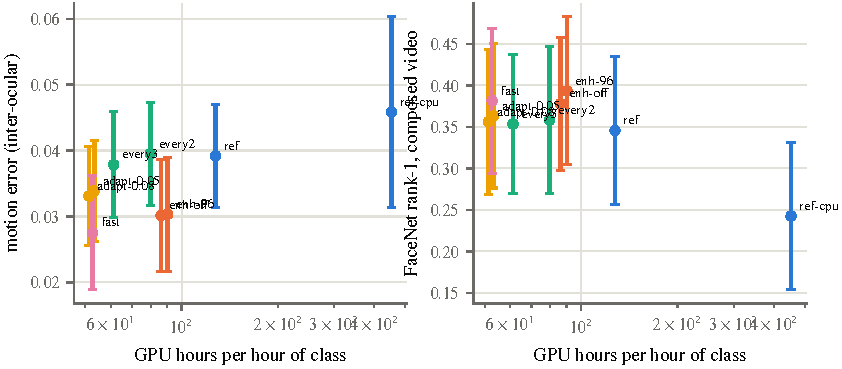
\includegraphics[width=\linewidth]{generated/e5_cost/fig-e5-tradeoff}
\caption{E5: GPU-horas por hora de aula, FaceNet rank-1, $\kappa$ e movimento no vídeo composto, por braço.}
\end{figure}
